\documentclass[12pt,letterpaper,onecolumn]{article}
\usepackage{mathptmx}
\newcommand{\titlefont}{\fontfamily{ptm}\fontseries{b}\fontsize{16pt}{\baselineskip}\selectfont}
\newcommand{\authorfont}{\fontfamily{ptm}\fontseries{b}\fontsize{14pt}{\baselineskip}\selectfont}
\newcommand{\zwfont}{\fontfamily{ptm}\fontsize{12pt}{\baselineskip}\selectfont}
\newcommand{\codefont}{\fontfamily{phv}\fontsize{11pt}{\baselineskip}\selectfont}
\newcommand{\majorhead}{\fontfamily{ptm}\fontseries{b}\fontsize{12pt}{\baselineskip}\selectfont}
\usepackage{geometry}
\geometry{left = 1.0in,right = 1.0in,top = 1.0in,bottom = 1.0in}
\title{\titlefont Report for Lab 1}
\author{\authorfont Muhan Li,Man Sun,Mingxiao An}
\date{}
\begin{document}
	\maketitle
	\tableofcontents
	\section*{\majorhead Abstract}	
	%	The abstract should provide a brief overview of the report - one paragraph at most. 
	%	
	%	It should provide a summary of the main specific points for the introduction, the main tests and experiments, the results, and the conclusions. It is called an abstract because you can literally "abstract" sentences from the other sections. 
	%	
	%	Once again, this is not a narrative of your experiences as you executed the design.  The abstract should mirror (albeit in a very condensed way) the content of your report.	
		In this report, we will give a brief introduction on the purpose and tools used in the lab, a very detailed discussion of the lab. the testplan we will apply, the result of the lab as well as its analysis, the errors we met when doing this lab and the analysis, and the summary and conclusions of the whole lab and report. We will also hard copy our code used in this lab to the Appendices.
	\section*{\majorhead Introduction}
	%	Brief introduction and overview of the purpose of the lab and of the methods and tools used - one to two paragraphs at most.
		This lab is the first lab of EE300. It provided a chance for students to get familiar with the develop environment, developing with C and Arduino and the lab kits they are going to use in the whole quarter. In detail, they will need to use the provided kits and Arduino to learn how to make an LED blink correctly, how to control the LED with a button brick, how to send information to serial monitor on the PC, how to work with LCD as well as control it, how to communicate between two microprocessors by I2C ,and finally, how to control a microprocessor's LED by another's button. The tools used in this lab are the Arduino IDE and the Arduino UNO microprocessor board.
	\section*{\majorhead Discussion of the Lab}
	%	This section should include the following:
	%	
	%	Brief Design Specification - In this subsection you will textually describe your client's requirements.  What does he or she need in the project you are developing.  If you are incorporating extra features or capabilities, please describe them clearly in this section.
	%	
	%	Overall summary description of the module - 2-3 paragraphs maximum
	%	
	%	Specification of the public interface to the module
	%	
	%	Inputs
	%	Outputs
	%	Side effects - what outside variables did the module change
	%	
	%	Pseudo English description of algorithms, functions, or procedures
	%	Error handling
	%	
	%	Hardware Implementation
	%	
	%	Draw the schematic / logic diagram of how you connected the parts...switches, chips, LEDs etc.
	%	
	%	Use standard symbols for simple electronic parts and appropriately labeled boxes for larger parts. Should be a cleaned-up "picture" of what your breadboard and components actually look like
	%	
	%	Do not actually take a picture and submit this.
	%	
	%	Software Implementation
	%	
	%	What is your design????
	%	
	%	Present your design starting from a top level functional view and potentially block diagram or high level architecture. 
	%	
	%	Refine that view to present and explain each of the modules that comprise the major functional blocks. 
	%	
	%	Discuss the flow of control through the design. 
	%	
	%	Identify and discuss the specific modules you have implemented in your design. Explain your design choices.    
		\subsection{Brief Design Specification}
\subsubsection{Overall summary description of the module}
Part 1 of the lab requires us to blink LEDs, and control its pattern by programs or a button. A communication between Arduino board and computer is also covered. To meet this requirment, we need to set the pins and their modes correctly, then program the processor to receive input, control the flow, and send output. Besides, we need to set up the connection between processor and computer. Test text will be sent to ensure it works correctly, and then the processor should do a calculation and send the result.
In part 2, we will need a module that can work with the LCD and two modules that can communicate, which reflects on the control of the LED of one microprocessor by another. To meet the requirement of being able to work with the LCD, we need the correct control of the content, situation, and moving of the characters printed on the LCD by the module. To meet the requirement of being able to communicate, we need to send data correctly from the master microprocessor to the slaver microprocessor.
\subsubsection{Specification of the public interface to the module}

\paragraph{Input, Output and Side Effects}
\subparagraph{lab 1 \& 2}
There is no input in this program. The output is the blinking of LED on the board, which follows a pattern we set before. 
\subparagraph{lab 3 \& 4}
This part is much like the one above, with the output device here being an LED brick instead of onboard LED. It blinks in two ways under the control of the program.
\subparagraph{lab 5}
We have connected a button brick to the board so whether it is pushed or not becomes the input signal. The output is the blinking of the LED brick, which is controlled by the brick.
\subparagraph{lab 6 \& 7}
In this part we are trying to use the processor output, so output is the information through serial. Program 6 prints some preset words on the serial monitor and Program 7 prints our own stuff. There is no input.
\subparagraph{lab 8} 
No input is required, the output is the LCD connected to the microprocessor printing two names on the first row of the display and one on the second.
\subparagraph{lab 9}
The input is controlled by two peripheral buttons, which can generate high signal by being pressed, and the output is the cursor on the LCD display moving left if one of the button is pressed and to the right if the other is pressed. If the cursor meets the end of the two rows of the LCD display, it will show up at the first column of the second row and can be controlled again.
\subparagraph{lab 10}
No input is required, and the output is detected on the Serial Monitor on the PC. If the Serial Monitors of the two microprocessors are opened separately, the slaver's monitor should display the same number series as the master's does. 
\subparagraph{lab 11}
The input is controlled by a peripheral button brick connected to the master microprocessor, and the output is the peripheral LED connected to the slaver microprocessor being turned on when the button is pressed, and turned off when the button is released.
\paragraph{Pseudo English description of algorithms, functions, or procedures}
\subparagraph{lab 1 \& 3}
set LED as output;
loop while true\{
	set the voltage high;
	wait for 2 seconds;
	set the voltage low;
	wait for 1 second;
\}
\subparagraph{lab 2 \& 4}
set LED as output;
loop while true\{
	two-second blink;
	one-second blink;
	two-second blink;
	two-second blink;
\}
\subparagraph{lab 5}
set LED as output;
set button as input;
loop while true\{
	if (button pushed)\{
		LED on;
	\}
	else\{
		LED off;
	\}
\}
\subparagraph{lab 6}
set an integer;
start serial port;
loop while true\{
	serial print "hello world";
	serial printline i;
	wait 1 second;
	serial printline "how ya doin";
	wait 1 second;
\}
\subparagraph{lab 7}
start serial port;
serial printline some own stuff;
\subparagraph{lab 8}
print the name of first two members;
move the cursor to the first column of the second row;
print the name of the third member;
\subparagraph{lab 9}
row = 0;col = 0;
connect the input pins to variables respectively;
if the variable related to the left button is high, and if cursor is at the beginning of the second row, move the cursor to the end of the first row, if it is at the beginning of the first row, do nothing, else col -=1 ;
if the variable related to the right button is high, and if cursor is at the end of the second row, move the cursor to the beginning of the second row, if it is at the end of the first row, move it to the beginning of the second row, else col +=1 ;
keep doing the checking process with a delay of 300 in each round;
\subparagraph{lab 10}
Although the code for this lab is provided on the course website, we will still present the pseudo code.
x = 0;
set the correct output port;
send the value of x ; x��+= 1;
keep the sending and adding process, with a delay in each round;
\subparagraph{lab 11}
lightOn = 0;
connect the variable lightOn to the control pin of the LED light in the slaver module;slaver module keeps receiving the signal from the master microprocessor and saves its correspondent value into lightOn.
if the button is pressed, the master sends a byte string representing that the light is on to the slaver, if not, it sends a byte string representing that the light is off to the slaver.
\subsection{Hardware Implementation}
\begin{figure}
	\centering
	\label{fig:1}
	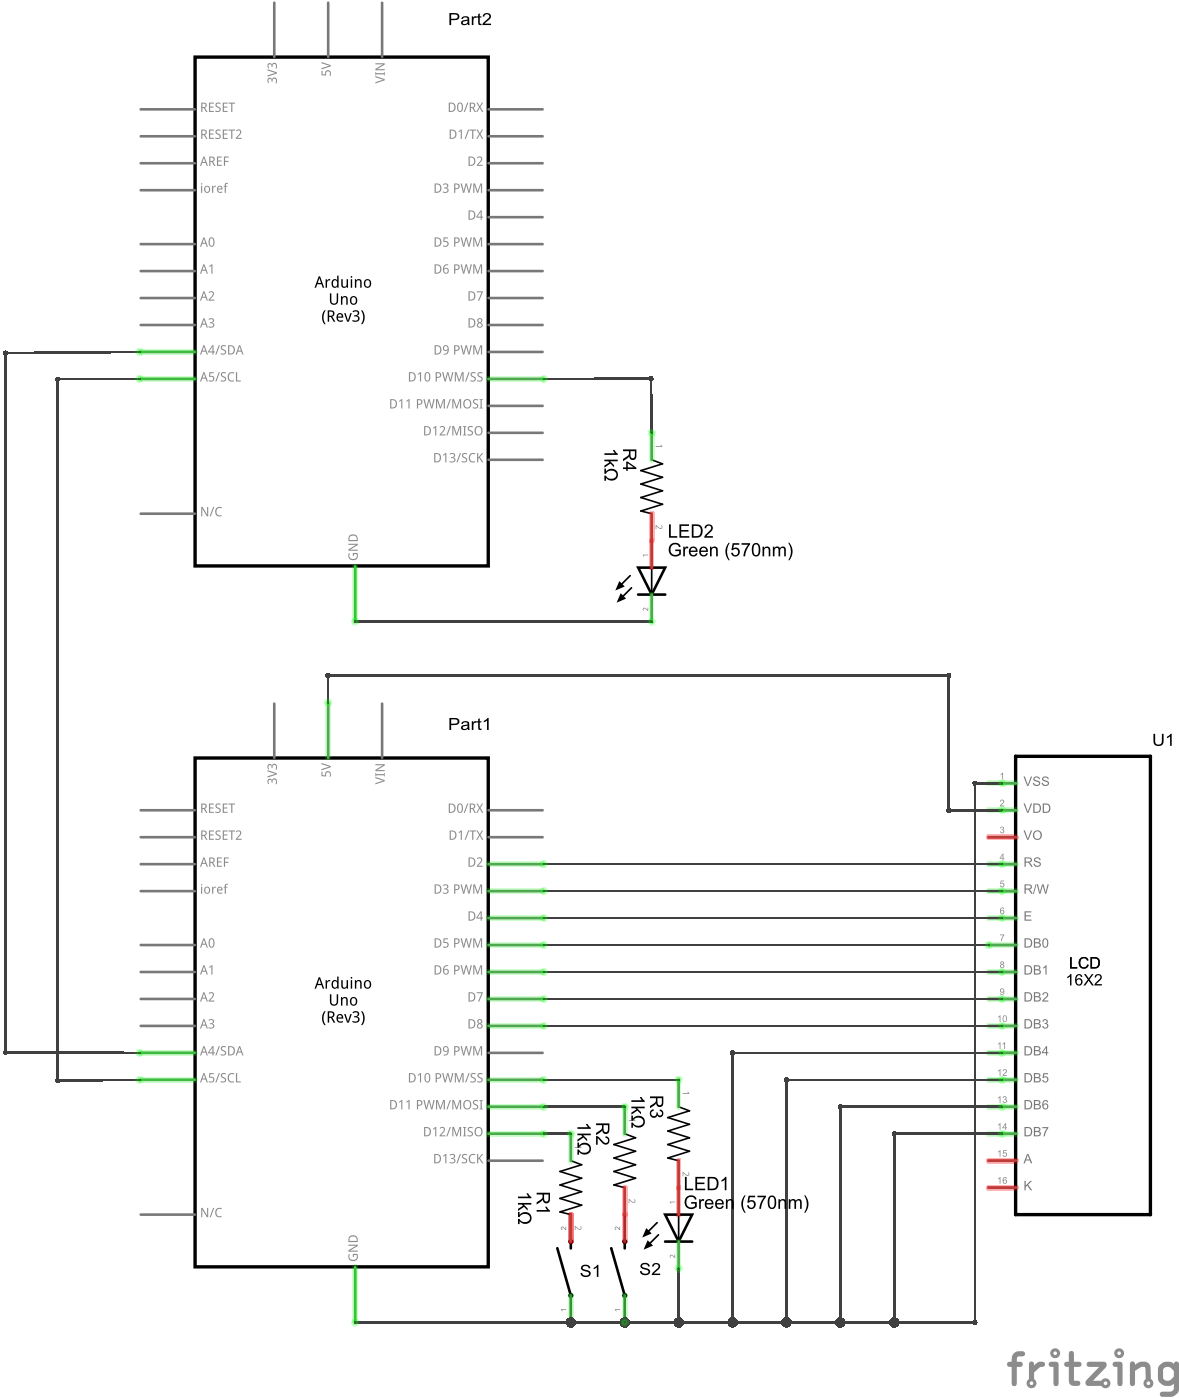
\includegraphics[width = \linewidth]{images/harware_schem.png}
	\caption{Schematic of hardware implementation(developed using Fritzing)}
\end{figure}
%\subsection{Software Implementation}
	\section*{\majorhead Testplan}
	%	Overall summary of what needs to be tested to ensure that your design meets the original requirements, 2-3 paragraphs maximum unless specified otherwise   
		\paragraph{Testplan for part 1}
	In part 1 of the lab, we learnt to use the laboratory and development environment, a combination of the traditional PC, Visual Studio, the Arduino UNO microcontroller and peripheral devices, and the Arduino integrated development environment (IDE), and how to work with a basic Blink program. The Blink program required us to make a LED light blink and use Arduino code and a button to control it. This requirement also contained being able to connect several peripherals, in this part a button and a LED, to the microprocessor. And finally we need to send output from a simple program to a display device, the Serial Monitor. So we will need to test if the blink statue of the controlled light meets the requirement, and if the output is correctly send to the Serial Monitor.\\
\paragraph{Testplan for part 2}
	In part 2 of the lab, we learnt to work with another display device, the LCD, and how to send information from one microprocessor, over a very simple network, to a second to control a peripheral device attached to the second microprocessor. Finally, we will need to control an LED of one microprocessor with another. As a result, we will need to test if the LCD can display correctly under our control, and if the two microprocessor can communicate correctly, and the LED light can be controlled from another microprocessor correctly.\\
	\section*{\majorhead Presentation, Discussion, and Analysis of the Results}
	%	Based upon the execution of your design, present your results. Explain them and what was expected, and draw any conclusions (for example, did this prove your design worked).
	%	
	%	In addition to a detailed discussion and analysis of your project and your results, you must include all the answers to all questions raised in the lab.
		\subparagraph{lab 8}
The names of the first two members are correctly shown on the first row of the display screen of the LCD connected to the microprocessor, and the name of the third member is correctly shown on the second row.
\subparagraph{lab 9}
The cursor on the screen of the LCD connected to the microprocessor can be incrementally moved by one space, left (by one button) or right(by another button). When the cursor meets the end of the first row, (if moved right), the cursor will move to the beginning of the second row. When the cursor meets the end of the second row,(if moved right), the cursor will move to the beginning of the second row.
\subparagraph{lab 10}
The serial monitors of the two microprocessors on the PC displays the same text series.
\subparagraph{lab 11}
The LED brick on slave can be turned ON and OFF by signals over I2C from a button brick on the master. When the button brick is pressed, the LED is turned On.
	\section*{\majorhead Analysis of any Errors}
	%	This one is obvious. Do this section as appropriate.  If it improves the flow, it does not need to be a separate section and may be included in the presentation, discussion, and analysis of the results.  However, it will still be graded separately and must be present.
		\subparagraph{lab 8}
We mistook A4 as D4 when we were building the circuit, but then we recognized it and correct our error.
We tried to use the BUS3 on the chassis at first(as the cookbook said), but it turned out that it is not working(we thought it wasn't connected to other circuits on the chassis board at all). So we used BUS1 instead, and it worked perfectly.
	\section*{\majorhead Analysis of Why the Project May not of Worked and What Efforts Were Made to Identify the Root Cause of any Problems}
	%	State any problems you encountered while working on the project. If your project did not work or worked only partially, provide an analysis of why and what efforts were made to identify the root cause of any problems. Should be written only if your project (or a required component) did not work. 
		\input{probs}
	\section*{\majorhead Summary and Conclusion}
	%	You should know these sections very well, no need to explain.  Note, however, that they are two different sections.  The summary is just that, a summary of your project.  It should loosely mirror the abstract with a bit more detail.  The conclusion concludes the report, potentially adds information that is often outside the main thrust of the report, and may offer suggestions or recommendations about the project.
		\paragraph{summary} In this report, we give a brief introduction on the purpose and tools used in the lab, a very detailed discussion of the lab. the testplan we will apply, the result of the lab as well as its analysis, the errors we met when doing this lab and the analysis, and the summary and conclusions of the whole lab and report. We will also hard copy our code used in this lab to the Appendices.
\paragraph{conclusions} We successfully complete our report and received an expected result. We also became familiar with the lab kits used in this lab, and also with the whole process of finishing a lab with Arduino and writing a corresponding report.
	\section*{\majorhead Appendices}
	%	Your final version of any and all pseudocode and C code should go in this section. 
		In this section, we will show all of our Arduino code that were developed and used in this lab.
\lstset{language=C}
\begin{lstlisting}[caption = blink1.ino]
// Pin 13
int led = 13;

// the setup routine runs once when you press reset:
void setup() 
{                
	// initialize the digital pin as an output.
	pinMode(led, OUTPUT);     
}

// the loop routine runs over and over again forever:
void loop() 
{
	digitalWrite(led, HIGH);   // turn the LED on (HIGH is the voltage level)
	delay(2000);               // wait for two seconds
	digitalWrite(led, LOW);    // turn the LED off by making the voltage LOW
	delay(1000);               // wait for a second
}
\end{lstlisting}
\begin{lstlisting}[caption = blink2.ino]
// Pin 13 
int led = 13;

// the setup routine runs once when you press reset:
void setup() 
{                
	// initialize the digital pin as an output.
	pinMode(led, OUTPUT);     
}

// the loop routine runs over and over again forever:
void loop() 
{
	digitalWrite(led, HIGH);   // turn the LED on (HIGH is the voltage level)
	delay(1000);               // wait for a second
	digitalWrite(led, LOW);    // turn the LED off by making the voltage LOW
	delay(1000);               // wait for a second
	digitalWrite(led, HIGH);   // turn the LED on (HIGH is the voltage level)
	delay(1000);               // wait for a second
	digitalWrite(led, LOW);    // turn the LED off by making the voltage LOW
	delay(1000);               // wait for a second
	
	digitalWrite(led, HIGH);   // turn the LED on (HIGH is the voltage level)
	delay(2000);               // wait for two seconds
	digitalWrite(led, LOW);    // turn the LED off by making the voltage LOW
	delay(1000);               // wait for a second
	digitalWrite(led, HIGH);   // turn the LED on (HIGH is the voltage level)
	delay(2000);               // wait for two seconds
	digitalWrite(led, LOW);    // turn the LED off by making the voltage LOW
	delay(1000);               // wait for a second
}
\end{lstlisting}
\begin{lstlisting}[caption = blink3.ino]
// LED Pin 8
int led = 8;

// Button Pin 9
int button = 9;

// the setup routine runs once when you press reset:
void setup() 
{
	// initialize the digital pin as an output.
	pinMode(led, OUTPUT);     
	// 
	pinMode(button, INPUT);
}

// the loop routine runs over and over again forever:
void loop() 
{
	if (digitalRead(button)) 
	{
		digitalWrite(led, HIGH);   // turn the LED on (HIGH is the voltage level)
	} 
	else 
	{
		digitalWrite(led, LOW);   // turn the LED off
	}
}
\end{lstlisting}
\begin{lstlisting}[caption = LCD1.ino]
#include <LiquidCrystal.h>

LiquidCrystal lcd(2, 3, 4, 5, 6, 7, 8); // Bus 1

void setup() 
{
	lcd.begin(16, 2); // 16 * 2 character
	
	lcd.print("Man Muhan");
	lcd.setCursor(0, 1);
	lcd.print("Mingxiao");
}

void loop() 
{
	// do nothing
}
\end{lstlisting}
\begin{lstlisting}[caption = LCD2.ino]
#include <LiquidCrystal.h>

LiquidCrystal lcd(2, 3, 4, 5, 6, 7, 8); // port 1
int buttonLeft = 10;
int buttonRight = 9;
int col = 0;
int row = 0;


void moveLeft() 
{
	lcd.clear();
	if (col > 1) col -= 1;
	else if (row > 0) 
	{
		row -= 1;
		col = 16;
	}
	lcd.setCursor(col, row);
	lcd.print("X");
}

void moveRight() 
{
	lcd.clear();
	if (col < 16)
	col += 1;
	else 
	{
		row += 1;
		col = 1;
	}
	lcd.setCursor(col, row);
	lcd.print("X");
}

void setup() 
{
	pinMode(buttonLeft, INPUT);
	pinMode(buttonRight, INPUT);
	lcd.begin(16, 2); // 16 * 2 character
	lcd.autoscroll();
	//  lcd.cursor();
	moveRight();
}

void loop() 
{
	if (digitalRead(buttonLeft)) 
	{
		moveLeft();
		delay(300);
	}
	if (digitalRead(buttonRight)) 
	{
		moveRight();
		delay(300);
	}
}
\end{lstlisting}
\begin{lstlisting}[caption = 12i2cm.ino]
#include <Wire.h>

void setup()
{
	Wire.begin();         // join i2c bus (address optional for master)
	Serial.begin(9600);       // start serial for output
}

byte lightOn = 1;

void loop()
{
	Wire.beginTransmission(4);  // transmit to device #4
	Wire.write(lightOn);      // send the signal of whether the LED is on
	
	Wire.endTransmission();     // stop transmitting
	if(lightOn == 1)
	{
		Serial.print("LED on\n");
		lightOn = 0;
	}
	else 
	{
		Serial.print("LED off\n");
		lightOn = 1;
	}
	delay(500);
}
\end{lstlisting}
\begin{lstlisting}[caption = 12i2cs.ino]
#include <Wire.h>
// Pin 13
int led = 13;
void setup()
{
	Wire.begin(4);         // join i2c bus with address #4
	Wire.onReceive(receiveEvent); // register event
	Serial.begin(9600);       // start serial for output
	pinMode(led,OUTPUT);
}
void loop()
{
	delay(100);
}
// function that executes whenever data is received from master
// this function is registered as an event, see setup()
void receiveEvent(int howMany)
{
	while(1 <Wire.available())  // loop through all but the last
	{
		Serial.print("received");
		bool on = Wire.read();    // receive byte as a character
		if(on)
		{
			digitalWrite(led,HIGH);
			Serial.print("LED on\n");
		}
		else
		{
			digitalWrite(led,LOW);
			Serial.print("LED off\n");
		}
	}
}
\end{lstlisting}
		
\end{document}